\chapter{Diseño y ensamblado}
\label{ch:DisenoEnsamblado}

En esta sección se describirán los pasos necesarios para la concreción física
del proyecto.
Se comienza con la confección e interpretación del diagrama de tuberías e
instrumentación, con el objetivo de detallar la solución propuesta en
la Sec. \ref{sec:SolucionPropuesta}.
Luego se hará énfasis en la construcción de la planta a partir de los elementos
disponibles.
Se describirá en detalle cada uno de ellos y se hará mención de
las decisiones constructivas tomadas durante el ensamblado.

\section{Diagrama de tuberías e instrumentación - P\&ID}
\label{sec:p&id}

\subsection{Generalidades}
Un diagrama de tuberías e instrumentación es un esquema de la planta en donde
pueden observarse todos los elementos que componen el proceso.
Estos diagramas emplean símbolos para representar cada elemento y sus
conexiones.
Los símbolos están regidos por la norma
\emph{ISA 5.1}.

El diagrama permite una rápida comprensión del proceso, y se denomina
corrientemente \gls{pyid}.

En los diagramas \gls{pyid} se encuentran graficados los diferentes elementos
como círculos o símbolos representativos, cada uno de ellos acompañado de una
denominación que utiliza la siguiente codificación:

\begin{itemize}  
 \item \textbf{Primer letra:}
 designa la variable medida o de interés. Puede ser, entre muchas otras:
 \begin{itemize}
  \item Presión
  \item Nivel
  \item Caudal
  \item Temperatura
 \end{itemize}

 \item \textbf{Letras siguientes:}
 designa la función del componente, o modifica el sentido de la primer letra.
 Puede ser:
 \begin{itemize}
  \item Indicador
  \item Registro de datos
  \item Controlador
  \item Transmisor
  \item Alarma
 \end{itemize}
\end{itemize}

Así mismo, estos círculos pueden estar intersectados por una línea, la
cual
indica su ubicación:

\begin{itemize}
 \item \textbf{Sin línea:} en el campo.
 \item \textbf{Continua:} en la sala de control.
 \item \textbf{Trazos:} fuera del alcance del operario, por ejemplo, en tablero
secundario o auxiliar.
\end{itemize}

Como su nombre lo indica, también están presente en el diagrama la descripción
de las tuberías que forman el sistema (material, diámetros y condiciones de
operación, en términos de temperatura y presión).
Cabe destacar que en esta instancia no es necesario especificar las
longitudes y accesorios.
Esta información forma parte de un diagrama que se debe realizar
en una etapa posterior del proyecto.

También se diferencian en el diagrama la naturaleza de cada señal:

\begin{itemize}
 \item \textbf{Tubería:} línea continua.
 \item \textbf{Señal hidráulica:} línea continua intersectada con líneas
perpendiculares en forma de L.
 \item \textbf{Señal neumática:} linea continua intersectada por pequeñas
líneas paralelas e inclinadas.
 \item \textbf{Señal eléctrica:} línea de trazos.
\end{itemize}

\subsection{P\&ID de la planta}
De acuerdo a los componentes detallados en la Sec.
\ref{sec:MaterialesDisponibles} se realizó el esquema \gls{pyid} de la planta
de control de nivel.
Para la correcta comprensión de este capítulo es indispensable contar con el
esquema, que puede observarse en la Fig. \ref{img:pyid}.

\begin{figure}
	\centering
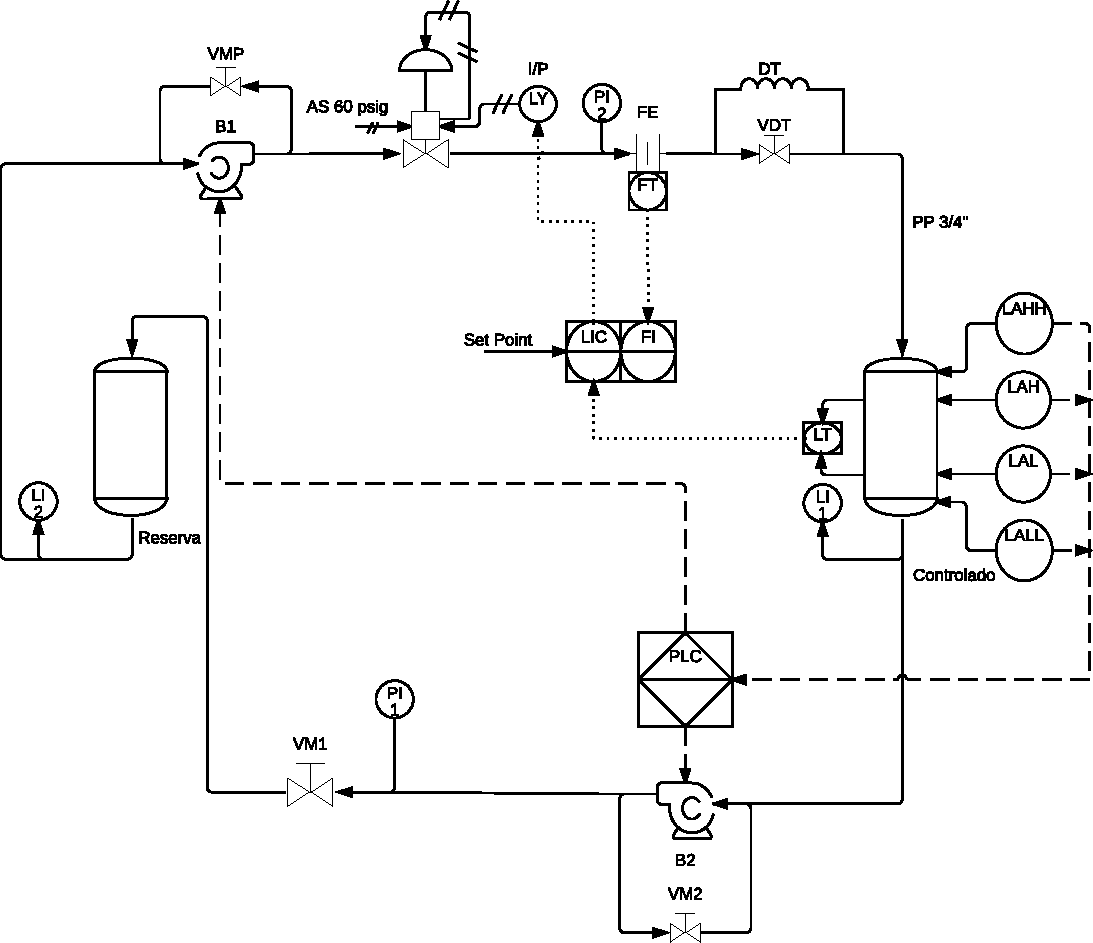
\includegraphics[width=\textwidth]{Cap2-DisenoEnsamblado/images/pyid60-1.pdf}
	\caption{Diagrama P\&ID del proyecto}
	\label{img:pyid}
\end{figure}

Las diferentes partes del diagrama se explicarán a continuación:

\subsubsection{Líneas}

\begin{itemize}
 \item \textbf{Línea de trazos:} $24\,V$.
 \item \textbf{Línea de puntos:} $4$ - $20\,mA$.
 \item \textbf{Línea continua:} tubo de polipropileno de 3/4 pulgada.
\end{itemize}

\subsubsection{Elementos}

En la Tab. \ref{tab:elementos} se presentan los símbolos de
los elementos que forman parte del diagrama \gls{pyid}, como así
también se detalla el significado de las siglas.

\begin{table}[h]
\small
\centering
\renewcommand*{\arraystretch}{0.3}

\begin{tabular}{*{2}{m{0.435\textwidth}}}
\hline
Tanque e indicador de nivel en tanque

LI: Level Indicator
  &\begin{center}
    %\rule{0.4\textwidth}{0.3\textwidth}
    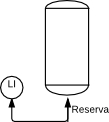
\includegraphics[scale=.5]
	{Cap2-DisenoEnsamblado/images/tanque.png}
  \end{center}\\
\hline
Bomba centrífuga
  &\begin{center}
    %\rule{0.4\textwidth}{0.3\textwidth}
    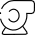
\includegraphics[scale=.55]
	{Cap2-DisenoEnsamblado/images/bomba.png}
  \end{center}\\
\hline
Válvula neumática
  &\begin{center}
    %\rule{0.4\textwidth}{0.3\textwidth}
    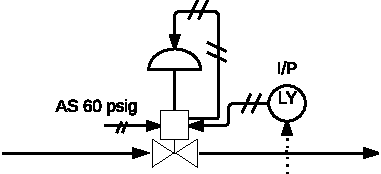
\includegraphics[scale=.5]
	{Cap2-DisenoEnsamblado/images/ValvPyID.pdf}
  \end{center}\\
\hline
Placa orificio y DP Cell.

FT: Flow Transmitter
  &\begin{center}
    %\rule{0.4\textwidth}{0.3\textwidth}
    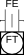
\includegraphics[scale=.5]
	{Cap2-DisenoEnsamblado/images/placa.png}
  \end{center}\\
\hline
Tiempo muerto

DT: Dead Time
  &\begin{center}
    %\rule{0.4\textwidth}{0.3\textwidth}
    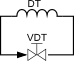
\includegraphics[scale=.5]
	{Cap2-DisenoEnsamblado/images/tmuerto.png}
  \end{center}\\
\hline
Controlador

LIC: Level Indicator and Controller

FI: Flow Indicator
  &\begin{center}
    %\rule{0.4\textwidth}{0.3\textwidth}
    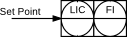
\includegraphics[scale=.5]
	{Cap2-DisenoEnsamblado/images/controlador.png}
  \end{center}\\
\hline
Transmisor e indicador de nivel

LI: Level Indicator

LT: Level Transmitter
  &\begin{center}
    %\rule{0.4\textwidth}{0.3\textwidth}
    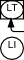
\includegraphics[scale=.5]
	{Cap2-DisenoEnsamblado/images/tnivel.png}
  \end{center}\\
\hline
Válvula e indicador de presión

PI: Pressure Indicator
  &\begin{center}
    %\rule{0.4\textwidth}{0.3\textwidth}
    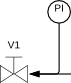
\includegraphics[scale=.5]
	{Cap2-DisenoEnsamblado/images/valvulam.png}
  \end{center}\\
\hline
\end{tabular}
\caption{Elementos del diagrama P\&ID}
\label{tab:elementos}
\end{table}

\subsubsection{Alarmas} 
\label{subsec:alarmas}

La gestión de alarmas se realiza a través del transmisor LT presente
en la planta,
tomando la información del mismo para detener el sistema en caso de pasar
los límites normales de trabajo.
Este proceso debería realizarse utilizando sensores
discretos, tipo level switch, separados.
No obstante, debido al costo de incluir sensores suplementarios,
se decidió utilizar
directamente el transmisor analógico de nivel y extraer de él
los valores de disparo, ya sean de alarmas como de paros.

En la Tab. \ref{tab:alarmas} se presenta la descripción de cada símbolo de
alarma.

\begin{table}[h]
\small
\centering
\renewcommand*{\arraystretch}{0.3}

\begin{tabular}{*{2}{m{0.435\textwidth}}}
\hline
LAHH: Level Alarm High High (paro por alto nivel)
  &\begin{center}
    %\rule{0.4\textwidth}{0.3\textwidth}
    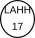
\includegraphics[scale=.7]
	{Cap2-DisenoEnsamblado/images/lahh.png}
  \end{center}\\
\hline
LAH: Level Alarm High
  &\begin{center}
    %\rule{0.4\textwidth}{0.3\textwidth}
    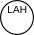
\includegraphics[scale=.7]
	{Cap2-DisenoEnsamblado/images/lah.png}
  \end{center}\\
  \hline
LAL: Level Alarm Low
  &\begin{center}
    %\rule{0.4\textwidth}{0.3\textwidth}
    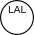
\includegraphics[scale=.7]
	{Cap2-DisenoEnsamblado/images/lal.png}
  \end{center}\\
\hline
LALL: Level Alarm Low Low (paro por bajo nivel)
  &\begin{center}
    %\rule{0.4\textwidth}{0.3\textwidth}
    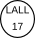
\includegraphics[scale=.7]
	{Cap2-DisenoEnsamblado/images/lall.png}
  \end{center}\\
\hline
PLC: símbolo de la sección del programador encargado
de la gestión de alarmas
  &\begin{center}
    %\rule{0.4\textwidth}{0.3\textwidth}
    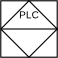
\includegraphics[scale=.6]
	{Cap2-DisenoEnsamblado/images/plc.png}
  \end{center}\\
\hline
\end{tabular}
\caption{Alarmas en el P\&ID}
\label{tab:alarmas}
\end{table}

\section{Estructura de soporte}
\label{sec:EstructuraSoporte}

Dado que el objetivo principal del proyecto es que la planta sirva para fines
educativos, se opta por utilizar una estructura móvil.
De esta manera, la ubicación de la planta puede modificarse según se requiera.

La estructura, de caño estructural, está dotada de cuatro ruedas con frenos de
seguridad, que permiten fijar la
planta al momento de una demostración.
Sus dimensiones se presentan en la Tab. \ref{tab:dimensionesEstructura}.

\begin{table}[ht]
\renewcommand{\arraystretch}{1.3}
\centering
\begin{tabular}{|l|l|}
\hline
Alto & $1.55\,m$ (incluido ruedas)\\
Ancho &  $1.50\,m$\\
Profundidad &  $0.52\,m$\\
\hline
\end{tabular}
\caption{Dimensiones de la estructura de soporte}
\label{tab:dimensionesEstructura}
\end{table}
 
La estructura presenta en su sección media barras de refuerzo.
Sobre ellas se colocaron los tanques.
Además, sobre las barras se fijó una base de madera, donde se coloca la
válvula de control, las celdas de presión diferencial
y las electrobombas.
La tubería flexible que corresponde al tiempo muerto se colocó bajo
las barras de refuerzo.
En la parte superior de la planta se instaló una pequeña base de
madera donde se montó el receptor inalámbrico.
Ya está incluida en la estructura el tablero, donde se
montaron los elementos eléctricos y electrónicos.
Sus dimensiones se observan en la Tab. \ref{tab:dimensionesTablero}.

\begin{table}[h]
\renewcommand{\arraystretch}{1.3}
\centering
\begin{tabular}{|l|l|}
\hline
Alto & $62\,cm$\\
Ancho &  $30\,cm$\\
Profundidad &  $20\,cm$\\
\hline
\end{tabular}
\caption{Dimensiones del tablero}
\label{tab:dimensionesTablero}
\end{table}

Al comienzo del proyecto la estructura de caño estaba ya soldada y pintada, con
las ruedas colocadas.
No obstante, el grupo de trabajo tuvo que barnizar las maderas.

\section{Tuberías}
\label{sec:Canerias}

\subsection{Tuberías flexibles y rígidas}
Luego de analizar el esquema \gls{pyid}, se observa que las tuberías deben
formar un circuito cerrado (\emph{loop}), diferenciando
claramente las tuberías de vaciado y llenado.
Las conexiones fueron realizadas en su mayoría utilizando tubo de polipropileno
de 3/4
pulgadas (presión de servicio: $11.7\,kgf/cm^2$ a $20^\circ C$).
En otros puntos del circuito, se optó por utilizar tubo flexible de alta presión
telado de 3/4 pulgadas (presión de servicio: $10\,kgf/cm^2$ a $20^\circ C$).
Las tuberías utilizadas son suficientes para las presiones de trabajo del
proyecto, del orden de $1.2\,kgf/cm^2$.

Habiendo montado los elementos sobre la planta (electrobombas, tanques, válvula
de control) se
decidió la manera de realizar el conexionado.
El tubo rígido presenta la dificultad de no tener tolerancia, al momento de
realizar uniones.
Además, para realizar tuberías rígidas complejas con muchas curvas, es necesario
colocar un gran número de componentes suplementarios (uniones dobles,
niples).
La planta se torna compleja, dificultando la comprensión del circuito
hidráulico por parte del alumno.
Es por ello que se optó por usar en diferentes secciones tuberías flexibles:

\begin{itemize}
  \item \textbf{Salida del tanque de reserva - entrada a la bomba B1}:
  se utilizo tubería flexible, dado que la estructura no permitía colocar tubos
  rígidos: los elementos de polipropileno necesarios eran más grandes que el
  espacio disponible.

  \item \textbf{Salida de la bomba B1 - entrada a la válvula:}
  se utilizo tubería flexible, para evitar una unión doble en un trayecto muy
  pequeño.
  
  \item \textbf{Salida de la válvula - entrada al tanque controlado:}
  debido a la longitud del tramo se optó usar tubos rígidos.
  Además, se montaron elementos de medición sobre la tubería (manómetro y
  placa orificio).
  
  \item \textbf{Salida del tanque controlado - entrada a la bomba B2:}
  debido al mismo problema de falta de espacio, se optó por el uso de tubería
  flexible.
  
  \item \textbf{Salida de la bomba - entrada al tanque de reserva:}
  esta conexión es la más larga y en ella van montados manómetros y
  válvulas manuales. Por ello, se prefirió la tubería rígida de polipropileno.

  \item \textbf{Conexión by-pass de las bombas:}
  se utilizó tubería flexible, para evitar uniones dobles y
  niples que requieren de una gran precisión durante el montaje.
 \end{itemize}

Por último se procedió a pintar los tubos mediante un código de colores.
 \begin{itemize}
  \item {\color{Cerulean} \textbf{Celeste:}} llenado del tanque controlado.
  \item {\color{YellowOrange} \textbf{Amarillo:}} vaciado del tanque controlado.
 \end{itemize}
El código de colores, si bien no es estándar en la industria, permite una fácil
comprensión del circuito hidráulico (ver Fig. \ref{fig:canerias}).

\begin{figure}[t]
        \centering
        \begin{subfigure}[b]{0.40\textwidth}
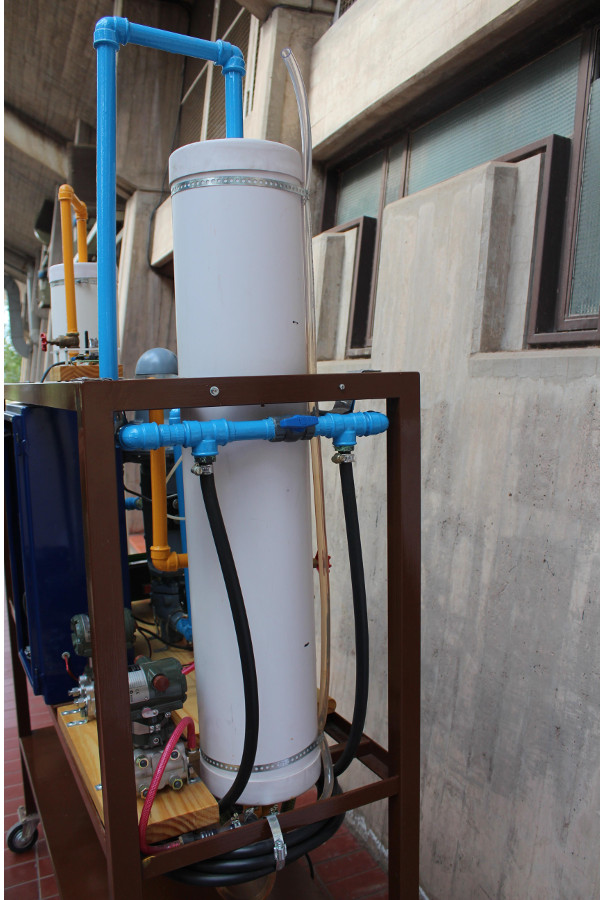
\includegraphics[width=\textwidth]
	{Cap2-DisenoEnsamblado/images/caneria1.JPG}
	\caption{Tubería de llenado}
        \end{subfigure}%
        \hfill
        \begin{subfigure}[b]{0.40\textwidth}
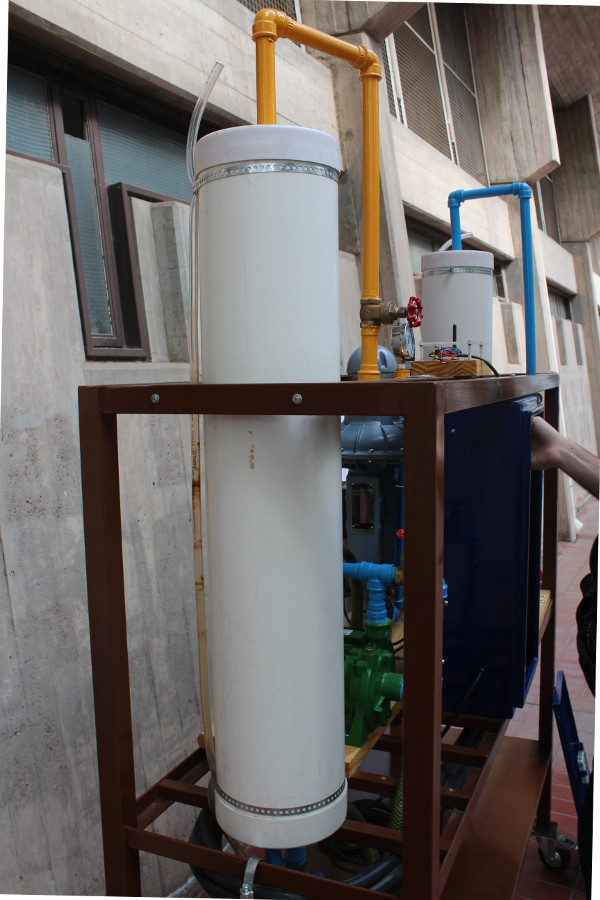
\includegraphics[width=\textwidth]{Cap2-DisenoEnsamblado/images/caneria2.JPG}
	\caption{Tubería de vaciado}
        \end{subfigure}
        \caption{Código de colores de las tuberías}
        \label{fig:canerias}
\end{figure}

\subsection{Tiempo muerto}
\label{subsec:tiempoMuerto}
Se colocó en la planta un circuito de tiempo muerto, que consta de 20 metros de
tubo semi rígido de 1/2 pulgada.
El tiempo muerto se coloca en paralelo de la tubería de llenado (ver
\gls{pyid}).
Mediante la válvula manual \verb|VDT| puede habilitarse el tiempo muerto.

El objetivo del tiempo muerto es alejar la acción de control del tanque
controlado.
El transmisor de nivel tardará un tiempo adicional $t_d$ en observar los cambios
que se producen en el actuador (válvula de control)
\cite{bib:ApuntesPuglesiTema2}.
La función de transferencia de la planta cambia notablemente:
\begin{itemize}
 \item Por un lado, el retraso en la respuesta debe ser tenido en cuenta
 \begin{align}
  G_{td}(s) &= e^{-t_d\,s}\,G(s)
 \end{align}
 donde $G(s)$ corresponde a la función de transferencia de una planta sin
 tiempo muerto, y $G_{td}(s)$ es la misma planta con tiempo muerto.
  \item Por otro lado, se agregan pérdidas por rozamiento del
  fluido cambiando la función de transferencia original $G(s)$ de la
  planta.
\end{itemize}
En conclusión, el proceso a controlar es diferente comparado con proceso sin
tiempo muerto.
La inclusión de este tubo semi rígido adicional permite disponer de dos
escenarios
diferentes para realizar prácticas, con la necesidad de contar con
controladores específicos para cada caso \cite{bib:ApuntesPuglesiTema2}.

\subsection{Válvulas manuales}

Diferentes válvulas manuales pueden encontrarse en las tuberías de la planta.
A continuación, se destacará la función de cada una de ellas:

\begin{itemize}
  \item \textbf{Desagote de los tanques:}
  para poder vaciarlos, se colocaron válvulas esféricas plásticas debajo de
cada tanque\footnote{Importante: estas válvulas no están dibujadas en el
\gls{pyid}.}.

  \item \textbf{Ecualización de la planta \texttt{VM1} y \texttt{VM2}:} se
colocó una válvula en serie con la tubería de retorno (ver
Fig.\ref{fig:valvTanque}).
Se trata de una
válvula manual, tipo exclusa.
Además, otra válvula manual del mismo tipo se coloca entre la tubería de
aspiración y
la tubería de impulsión de la bomba \verb|B2| formando un \emph{by-pass} (ver
Fig.\ref{fig:valvBomba}).
Al abrir la válvula, el rendimiento de la bomba decrece.
  Ambas válvulas permiten modificar el balance de masa y ecualizar la planta.

  \item \textbf{Tiempo muerto \texttt{VDT}:}
  tal como se describió en la Sec. \ref{subsec:tiempoMuerto}, esta válvula
esférica plástica permite activar la tubería de tiempo muerto.
  Notar en el \gls{pyid} que la válvula está sobre la tubería de llenado.
  Cerrando la válvula se fuerza el uso del tiempo muerto. Pero al
abrirla, nada impide que el fluido circule por las dos tuberías en paralelo.
  No obstante, la pérdida de carga del tiempo muerto es significativamente
mayor que el de la tubería de llenado.
  Por ello, se considera que el fluido circula únicamente por ésta última, al
abrir la válvula.

  \item \textbf{Perturbación \texttt{VMP}:}
  colocada de la misma manera que \verb|VM2|, pero sobre la bomba \verb|B1|.
  La válvula \verb|VMP| permite simular perturbaciones en la planta,
modificando el rendimiento de la bomba.

\end{itemize}

\begin{figure}[t]
        \centering
        \begin{subfigure}[b]{0.40\textwidth}
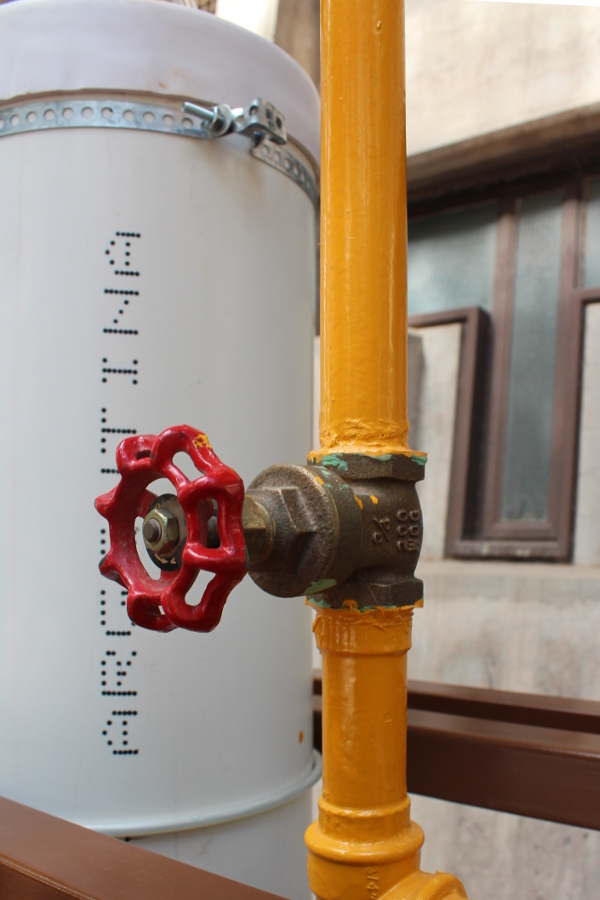
\includegraphics[height=8.5cm]{Cap2-DisenoEnsamblado/images/valvTanque.JPG}
                \caption{Control del caudal de vaciado}
                \label{fig:valvTanque}
        \end{subfigure}%
\hfill
        \begin{subfigure}[b]{0.40\textwidth}
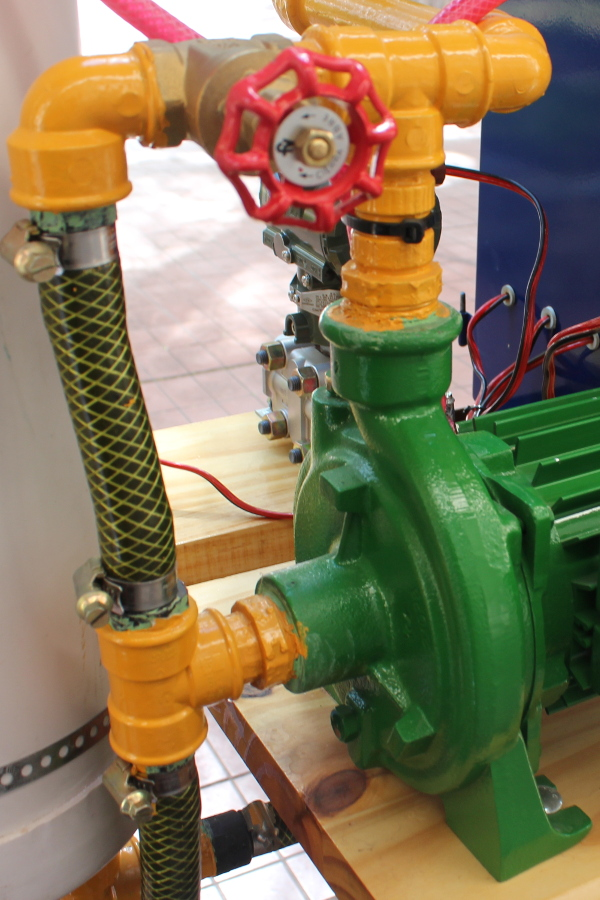
\includegraphics[height=8.5cm]{Cap2-DisenoEnsamblado/images/valvBomba.JPG}
                \caption{By-pass en bomba}
                \label{fig:valvBomba}
        \end{subfigure}
        \caption{Válvulas manuales en la planta}
        \label{fig:valvManuales}
\end{figure} 
 
\section{Tanques}
\label{sec:Tanques}

Los tanques almacenan el agua del sistema, y las acciones de
control están dirigidas a establecer el nivel presente en los mismos.
Se ubicaron en los extremos de la estructura, sobre las barras de 
refuerzo, fijándose a las barras laterales de la misma mediante
abrazaderas.

Son dos tubos cloacales de $200\,mm$ de diámetro y un metro de altura, que
fueron sellados en los extremos utilizando tapas.
La salida de agua hacia la tubería de aspiración de la bomba se realiza
mediante una conexión de tanque de 3/4 pulgada colocada en la base del tanque.
La entrada de agua se realiza por la parte superior, mediante un orificio
sencillo.

Además, en la base del tanque se colocó una segunda conexión de tanque de 3/4
pulgada, que se utiliza para medir el nivel.
Se conectan a esta tubería la celda de presión diferencial y un tubo
flexible transparente.
El tubo flexible, colocado en el lateral del tanque, permite obtener una
lectura visual directa del nivel.
Por otro lado, la celda de presión diferencial es un elemento de adquisición
que permite transformar un valor de presión (o su equivalente, altura de la
columna de agua a peso específico constante) en
una señal $4$-$20\,mA$.
Se discutirá sobre estos elementos en la Sec. \ref{subsec:DPCell}.

La tubería de aspiración de la bomba puede provocar
perturbaciones en la medición de la celda de presión diferencial.
Para evitar este problema, se optó por
colocar un niple en la conexión de aspiración, en el interior del tanque.
De esta manera, se separan físicamente ambas tuberías, reduciendo las
perturbaciones en la medición de presión.
Cabe destacar que la inclusión del niple limita el nivel mínimo de la planta a
un 15\% del nivel total, aproximadamente.

\section{Electrobombas}
\label{sec:Bombas}

Se utilizaron en el proyecto dos electrobombas centrífugas (\verb|B1| y
\verb|B2| en el \gls{pyid}), cuya función es
mantener en movimiento el agua en el sistema.
No se realiza ninguna acción de control sobre las
mismas, por lo que las bombas funcionan de manera continua durante la operación
de la planta.

Las bombas centrífugas son máquinas hidráulicas, que absorben energía mecánica
de un motor y la restituyen en forma de energía hidráulica al fluido.
En las bombas centrífugas (o radiales), esta ganancia de energía se realiza por
medio de la fuerza centrífuga que imparten los álabes del rodete de la bomba.
Este tipo de bomba se caracteriza por entregar una presión elevada y un caudal
relativamente bajo \cite{bib:Mataix}.

Las especificaciones de las electrobombas utilizadas se presentan en la Tab.
\ref{tab:caractBombas}.

\begin{table}[ht]
\renewcommand{\arraystretch}{1.3}
\centering
\begin{tabular}{|l|l|}
\hline
Marca & Czerweny\\
Caudal máximo &  $100\,l/min$\\
Altura máxima &  $12\,m = 1.2 kgf/cm^2$\\
Tensión & $220\,V$ monofásica $50\,Hz$\\
Corriente & $1.7\,A$\\
Seguridad & S1 IP44\\
\hline
\end{tabular}
\caption{Características de las electrobombas monofásicas}
\label{tab:caractBombas}
\end{table}

\subsection{Cavitación}
\label{subsec:cavitacion}
Para el ingreso del fluido a la bomba, es necesario realizar una succión
en la tubería de aspiración, descendiendo la presión del fluido.
Debido a la baja presión en la tubería de aspiración, el fluido puede
evaporarse formando burbujas de vapor.
Luego, la presión aumenta violentamente en el rodete de la bomba hasta alcanzar
la altura manométrica.
El rápido aumento de presión provoca una implosión de las burbujas.
Este fenómeno, conocido como \textbf{cavitación} genera ruido y disminuye la
vida útil de las las bombas \cite{bib:ApuntesMDFBombas}.

Para evitar la formación de burbujas de vapor, se opta por mantener la presión
en la tubería de aspiración lo más elevada posible.
Es por ello que las bombas se instalan en una posición baja.
Además, las bombas se colocaron lo más cerca posible de los respectivos
tanques disminuyendo las pérdidas en la tubería de aspiración.
Se fijaron mediante tornillos a la base de madera.

Durante la operación de la planta se observó un correcto funcionamiento de las
bombas, salvo cuando el by-pass se encuentra abierto en exceso: al
incrementar la
velocidad en la tubería de aspiración, la presión desciende llegando hasta el
punto de vapor.
Para evitar problemas de cavitación, se especifica en el anexo
\ref{anexo:verificaciones} el valor de apertura preciso para cada válvula.

\section{Válvula globo con servoactuador de diafragma - resorte y
electroposionador neumático}
\label{sec:ValvulaNeumatica}

En esta sección se hará énfasis en la válvula de control.
Es un elemento central en la planta, ya que es la encargada de efectuar
las acciones de control.

\subsection{Principio de funcionamiento}
\label{subsec:principioFuncionamiento}

\begin{figure}[t]
        \centering
        \begin{subfigure}[b]{0.37\textwidth}
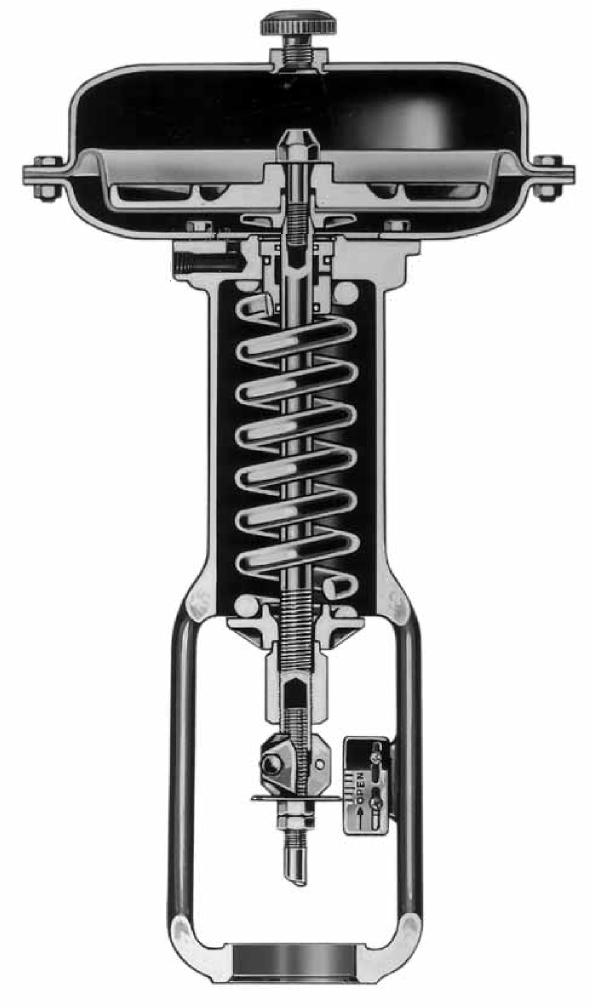
\includegraphics[width=\textwidth]
	{Cap2-DisenoEnsamblado/images/ActuadorValvNeum.png}
                \caption{Actuador neumático inverso}
                \label{fig:actuadorValv}
        \end{subfigure}%
        ~
        \begin{subfigure}[b]{0.37\textwidth}
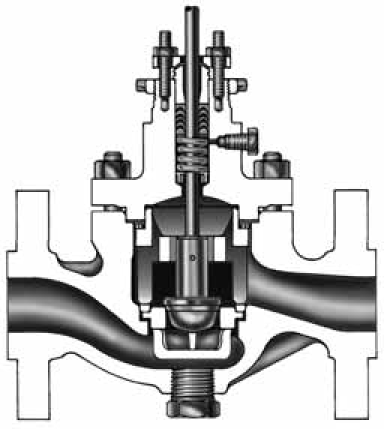
\includegraphics[width=\textwidth]{Cap2-DisenoEnsamblado/images/ValvGlob.png}
                \caption{Cuerpo de una válvula globo}
                \label{fig:cuerpoValv}
        \end{subfigure}
        \caption{Elementos constitutivos de una válvula neumática}
        \label{fig:elementosValv}
\end{figure}

Una válvula permite variar el caudal en una tubería, dependiendo de la consigna
que se le envíe.
En las válvulas neumáticas, la consigna es un valor de presión de aire sobre el
servoactuador.
En la Fig. \ref{fig:elementosValv} se muestra un ejemplo de válvula de control
tipo globo, con actuador a diafragma inverso (aire para
abrir)\footnote{Figuras extraídas de \cite{bib:controlValveHandbook}.}.
La válvula está compuesta de dos elementos principales: el actuador
(Fig. \ref{fig:actuadorValv}) y el cuerpo de la válvula (Fig.
\ref{fig:cuerpoValv}).

El obturador en el cuerpo de la válvula (Fig. \ref{fig:cuerpoValv}) apoya
sobre un asiento.
La variación del caudal se produce gracias al orificio de paso variable
que forman al variar su posición relativa el conjunto asiento-obturador.
Sobre el vástago, encargado de modificar la posición del obturador,
actúan las fuerzas del actuador.
Como se observa en la Fig. \ref{fig:actuadorValv}, el actuador en una válvula
neumática es el conjunto diafragma-muelle.

Puede concluirse, a través del análisis de la válvula, que el caudal depende de
la presión de aire sobre el servoactuador.
Generalmente, la presión oscila entre $3$ a $15\,psi$ (válvulas sin
electroposicionador) y $3$ a $30\,psi$ (válvulas con electroposicionador).
Esta presión de aire se obtiene mediante un convertidor
corriente-presión (I/P).
El convertidor toma en entrada una señal de corriente proveniente del
controlador
($4$ - $20\,mA$) y lo transforma en un valor de presión para alimentar el
servoactuador \cite{bib:ApuntesPuglesiValvulas}.

% \subsubsection{Rangeabilidad}
% Se denomina rangeabilidad a la razón entre el caudal máximo y el mínimo que
% puede controlar una válvula

\subsubsection{Tipos de obturador - Característica de caudal inherente}
Se denomina característica de caudal inherente a la variación del caudal de
la válvula en función de la carrera, manteniendo una presión diferencial
$\Delta p$ constante.
Para representar la característica inherente de una válvula, se grafica en
abscisas la carrera del obturador y en ordenadas el porcentaje de caudal máximo.

El conjunto asiento-obturador es la parte más importante de la válvula, ya que
es el elemento final que controla el caudal.
Dependiendo del tipo de conjunto asiento-obturador, se obtienen distintas
características de caudal inherente.
Se distinguen tres tipos:
\begin{itemize}
  \item \textbf{Obturador Lineal:} el caudal es proporcional a la carrera
  \begin{align}
	q = k\,l
	\label{eq:inherenteLineal}
  \end{align}
  donde $q$ es el caudal a pérdida de carga constante, $k$ es una constante y
$l$ es la carrera del vástago.

Se denomina rangeabilidad a la relación entre el caudal máximo y el caudal
mínimo que una válvula puede controlar ($q_{max}$ y $q_{min}$
respectivamente):
\begin{align}
 R &= \dfrac{q_{max}}{q_{min}}
 \label{eq:rangeabilidad}
\end{align}
La rangabilidad no es infinita:
aunque matemáticamente $q_{min}$ puede ser cero, según
\eqref{eq:inherenteLineal}, en la práctica la curva de caudal inherente no está
definida para valores de carrera próximos a cero.
Para una válvula lineal, $15 \leq R \leq 30$, debido a las dificultades
de fabricación \cite{bib:ApuntesPuglesiValvulas}.

  \item \textbf{Obturador Isoporcentual:}
  un incremento de carrera produce un cambio de caudal proporcional al caudal
que circulaba antes de la variación.
  \begin{align}
    \dfrac{dq}{dl} = a \, q
  \end{align}
  Operando, se puede reescribir esta expresión mediante una función exponencial
\begin{align}
 q = b\,e^{a\,l}
 \label{eq:InherenteIsoporcentual1}
\end{align}
  donde $a$ y $b$ son constantes para una válvula dada.
  Si se considera que
    \begin{align}
        l &= 0 \Rightarrow q = q_{min} = b\\
        l &= 1 \Rightarrow q = q_{max} = q_{min} \:e^a
    \end{align}
    puede escribirse
    \begin{align}
      \dfrac{q_{max}}{q_{min}} = e^a
    \end{align}
    Se puede reescribir la expresión
\eqref{eq:InherenteIsoporcentual1} como
\begin{align}
 q &= q_{min}  \left( {\dfrac{q_{max}}{q_{min}}} \right)^{l}
\end{align}
    y finalmente, basándonos en la expresión de rangeabilidad
\eqref{eq:rangeabilidad}, puede expresarse
    \begin{align}
     q &= \dfrac{1}{R}\, R^l \, q_{max}
    \end{align}
Para las válvulas isoporcentuales, $30 \leq R \leq 50$.
  \item \textbf{Obturador de apertura rápida:} permiten una brusca variación de
caudal con carreras pequeñas.
  No son utilizadas en el control regulatorio.
\end{itemize}

En la Fig. \ref{fig:caractInherente}, se grafican las curvas de caudal
inherente para cada tipo de válvula.
A simple vista, la válvula con obturador lineal ofrece las mejores
características para el control regulatorio.
No obstante, como se expondrá posteriormente, las curvas características de las
válvulas quedan afectadas por el proceso en el que se utilizan.

\begin{figure}[t]
 \centering
 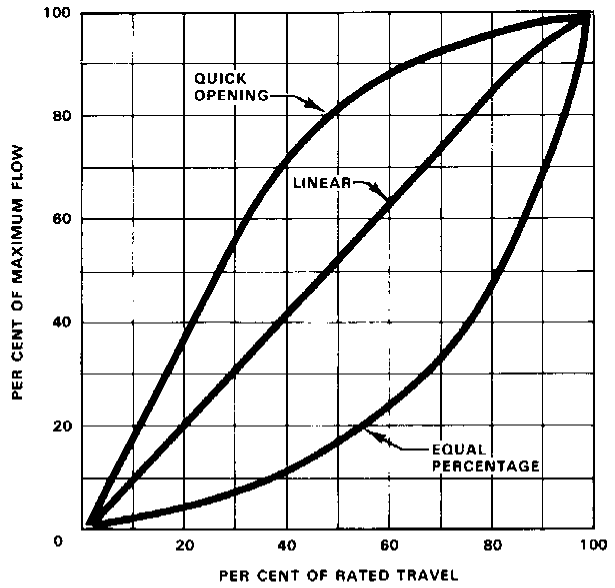
\includegraphics[scale=1.43]{Cap2-DisenoEnsamblado/images/Inherente.png}
 \caption{Características inherentes según el tipo de obturador}
 \label{fig:caractInherente}
\end{figure}


\subsubsection{Característica de caudal efectivas}

La característica de caudal inherente se traza para una presión diferencial
$\Delta \,p$ constante.
No obstante, en un proceso real, $\Delta \,p$ no es constante.
En efecto, las pérdidas de carga y la presión entregada por la bomba presentan
variaciones para diferentes caudales.

Se denomina característica de caudal efectiva a la variación del
caudal que atraviesa la válvula en función de su carrera, cuando la
válvula está inserta en un proceso real.
Dado que diferentes procesos proporcionan distintos valores de  $\Delta
\,p$, la característica de caudal efectiva depende del proceso.
Evidentemente, esta curva se aparta de la característica de caudal inherente,
como se demostrará a continuación.

En un circuito hidráulico, la presión que es entregada por la bomba $H$ se 
utiliza para vencer las pérdidas de carga en la tubería, contrapresiones y 
alturas (reagrupadas en $H_2$) y en la válvula.
Denotando $\Delta \,p = H_1$
\begin{align}
 H &= H_1 + H_2
\end{align}
$H_2$ varía cuadráticamente con el caudal según la ley de \emph{Darcy-Weisbach}
\cite{bib:Franzini}
\begin{align}
 H_2  &= f \dfrac{L}{D^5}\dfrac{16\,Q^2}{2\,g\,\pi^2} + H_c
\end{align}
donde $L$ es la longitud equivalente de la tubería, $D$ es el diámetro y $H_c$
representa la altura piezométrica (contrapresiones y alturas).
$H$ varía siguiendo la curva característica caudal-presión de la bomba.

Se denomina coeficiente $r$ a la razón entre la pérdida de carga de la válvula
$H_1$ comparado con la pérdida de carga total del sistema.
\begin{align}
 r &= \dfrac{H_1}{H_1+H_2} = \dfrac{H_1}{H}
\end{align}
Evidentemente, $r = 1$ cuando la tubería no tiene pérdida de carga,
aproximándose la característica efectiva a la inherente.
Puede demostrarse \cite{bib:Creus} que
\begin{align}
 q_e &= \dfrac{1}{\sqrt{1-r+\dfrac{r}{{q_i}^2}}}
 \label{eq:coef_r_qe_qi}
\end{align}
siendo $q_e$ el caudal efectivo y $q_i$ el caudal inherente, que puede
obtenerse mediante las ecuaciones \eqref{eq:inherenteLineal} y
\eqref{eq:InherenteIsoporcentual1}.

Puede concluirse, a partir de la ecuación \eqref{eq:coef_r_qe_qi} que la curva
de caudal efectivo varía dependiendo de $H_2$.
Si se grafican las características efectivas de diferentes tipos de válvulas,
se observa que al disminuir $r$ (pérdida de carga elevada) una válvula
isoporcentual tiende a comportarse como una lineal,
y una válvula lineal se comporta como de apertura rápida.


Dado que las válvulas de apertura rápida no son utilizadas en el control
regulatorio, se escoge entre una válvula isoporcentual o lineal dependiendo de
la pérdida de carga de la planta, con el objetivo de tener una característica
efectiva ``lo más lineal posible''.


\subsection{Válvula utilizada en el proyecto}

\begin{figure}[t]
        \centering
        \begin{subfigure}[b]{0.31\textwidth}
		\centering
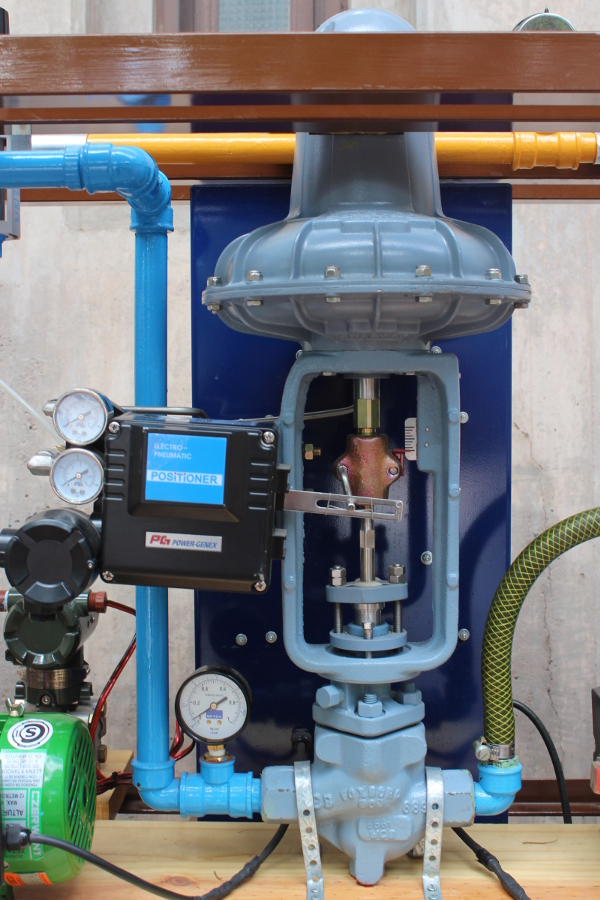
\includegraphics[height=6.3cm]{Cap2-DisenoEnsamblado/images/IMG_5129.JPG}
		\caption{Vista general de la válvula}
		\label{fig:fotoValvCompl}
        \end{subfigure}%
	\hfill
	\begin{subfigure}[b]{0.69\textwidth}
		\centering
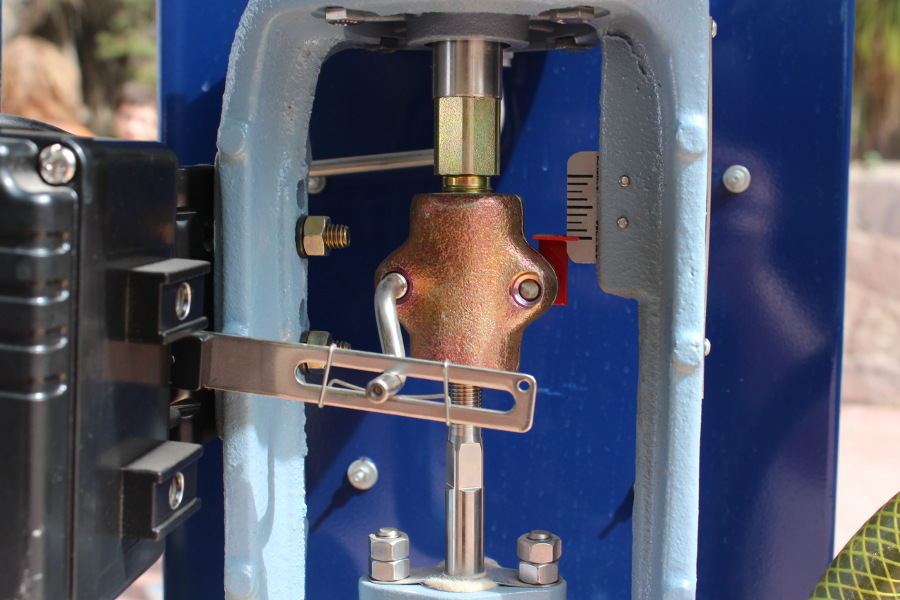
\includegraphics[height=6.3cm]{Cap2-DisenoEnsamblado/images/IMG_5030.JPG}
	\caption{Varilla de feedback e indicador de posición del vástago}
		\label{fig:fotoValvDetalle}
	\end{subfigure}%
	\caption{Válvula utilizada en el proyecto}
	\label{fig:fotoValv}
\end{figure}

En esta sección se describirán las características específicas de la válvula
utilizada en el proyecto (Fig. \ref{fig:fotoValv}), comparándolas con los
principios de funcionamiento
descriptos en la Sec. \ref{subsec:principioFuncionamiento}.

\subsubsection{Especificaciones}
Se muestran en la Tab. \ref{tab:especifValvs} las especificaciones más
importantes de la válvula, consignada en su chapa de identificación.

\begin{table}[ht]
\renewcommand{\arraystretch}{1.3}
\centering
 \begin{tabular}{|c|c|}
  \hline
  Marca & Foxboro\\
  Modelo & V1S-30CNTSSEBK-50\\
	& Stabilflo Serie V1\\
 Actuador & P-50 EA-DO\\
 Medida Cuerpo & 3/4 roscado\\
 Interior & Globo vástago\\
 Característica $C_v$ & $=\%\,CV=10$\\
 Temperatura & $-30$ a $207^\circ C$\\
 Aire para & Abrir  \\
 Carrera & $19\,mm$ \\
  \hline
 \end{tabular}
 \caption{Especificaciones de la válvula de control}
 \label{tab:especifValvs}
\end{table}

\subsubsection{Electroposicionador}
Se especificó que la presión de aire en el servoactuador varía entre $3\,psi$
(válvula cerrada) y $15\,-\,30\,psi$ (válvula abierta).
No obstante, en un convertidor I/P no hay comparación entre
la posición real del vástago y la señal de corriente.
Ciertos fenómenos como la fricción en el vástago, perturbaciones del fluido,
fuerzas dinámicas, etc. pueden modificar la apertura de la válvula.

Para paliar estos problemas, la válvula incluye un electroposicionador Power
Genex.
Se trata de un controlador proporcional que compara la posición actual del
vástago con la consigna de corriente.
En caso de detectar errores, ejerce la acción de control correctiva para
asegurar la posición del vástago.

\begin{figure}[t]
 \centering
 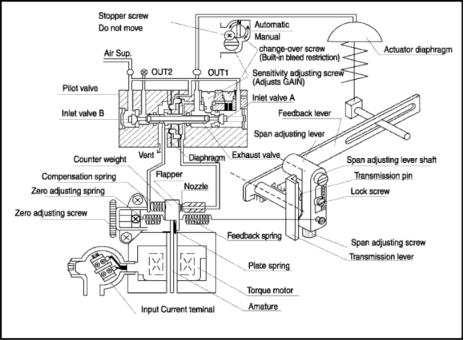
\includegraphics[scale=1.1]{Cap2-DisenoEnsamblado/images/PG-EPL.pdf}
 \caption{Esquema de funcionamiento del electroposicionador}
 \label{fig:elp-funcionamiento}
\end{figure}

En la Fig. \ref{fig:elp-funcionamiento} se muestra el esquema de
funcionamiento del electroposicionador.
La entrada de $4$-$20\,mA$ del controlador provoca una rotación en sentido
antihorario del motor de torque.
Lleva consigo al \emph{flapper}, liberando
presión por la boquilla (\emph{nozzle}) y moviendo la válvula hacia la
izquierda.
Se provoca un incremento de presión en \emph{OUT1} moviendo el diafragma del
actuador.

La varilla de feedback (\emph{feedback lever}, Fig. \ref{fig:fotoValvDetalle})
releva la posición del vástago y
la transmite mediante el resorte de feedback, que está vinculado con el
\emph{flapper}.
Se verifica que la posición del vástago de la válvula permanece constante
cuando el resorte de feedback iguala el par de rotación del motor de torque.
Otros elementos (\emph{compensation spring}, \emph{zero adjusting screw}) se
agregan para poder mejorar la estabilidad del bucle de control, como así
también poder calibrarlo\footnote{Explicación obtenida del manual del
electroposicionador.}.

La Tab. \ref{tab:especifElectroP} muestra las características más importantes
del electroposicionador presente en la planta.

\begin{table}[ht]
\renewcommand{\arraystretch}{1.3}
 \centering
 \begin{tabular}{|c|c|}
  \hline
  Marca & Power Genex\\
  Modelo & EPL-FA15N4TL\\
  Señal entrada & $4$-$20\,mA$ DC\\
  Presión de entrada & $1.4$ - $7\,bar$ máximo\\
  Temperatura de trabajo & $-20$a $70^\circ$\\
  Seguridad & Ex dmb IIB+H2 T6 IP66\\
  \hline
 \end{tabular}
 \caption{Especificaciones del electroposicionador}
 \label{tab:especifElectroP}
\end{table}

\subsubsection{Característica Efectiva de la válvula}

Como se describió en la Sec. \ref{subsec:principioFuncionamiento}, la
característica de caudal efectiva depende del proceso en donde la válvula esté
inserta. La característica de caudal efectiva puede encontrarse
experimentalmente:
\begin{enumerate}
 \item La planta se coloca en modo manual, encendiendo ambas bombas.
 \item Se coloca la válvula en una posición determinada enviando una consigna
de apertura manual.
 \item Se ecualiza la planta mediante las válvulas \verb|VM1| y \verb|VM2|. Se
trata de fijar el nivel de los tanques al 50\%.
 \item Establecido el nivel de la planta (sin oscilaciones) se realiza la
lectura en el DP cell del valor de la presión $h_p$,
y se calcula el caudal correspondiente (ver Sec. \ref{subsec:DPCell}).
 \item Se cambia la posición de la válvula en intervalos de
 10\%, desde el 0\% (totalmente cerrada) hasta el 100\% (totalmente abierta).
Se repite 3 a 5.
\end{enumerate}

Los resultados de esta experiencia en la planta se muestran en las Figs.
\ref{fig:valvulaStiempoMuerto} y \ref{fig:valvulaCtiempoMuerto}.
Puede apreciarse un comportamiento aproximadamente lineal de la válvula entre
$10\%$ y $70\%$ sin tiempo muerto, y entre $0\%$ y $60\%$ con tiempo muerto.
Luego, se produce un fenómeno de saturación conocido como flujo
estrangulado (\emph{choked flow}), que se discutirá posteriormente.
Se concluye que la válvula utilizada es adecuada para el
control regulatorio, debido a su característica efectiva aproximadamente lineal
en la zona de trabajo.

\begin{figure}[ht]
  \centering
  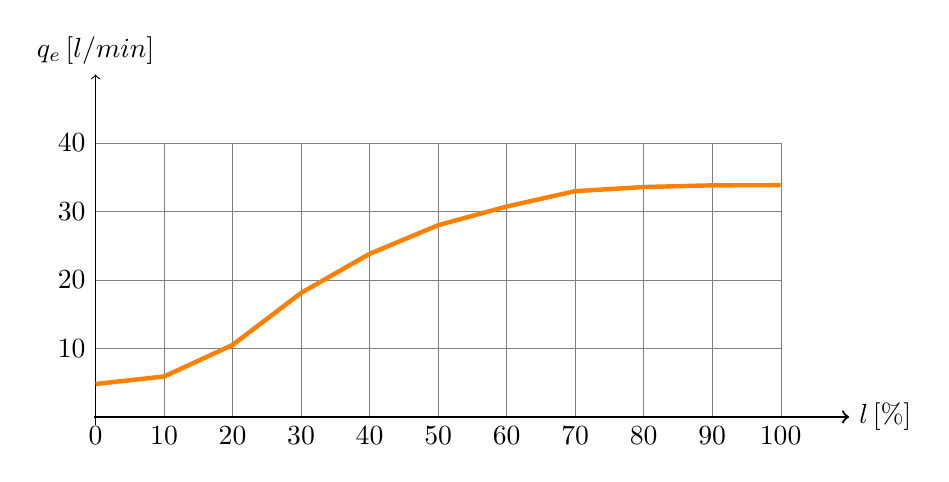
\begin{tikzpicture}[scale= 0.087, domain=0:110]
    
    \draw[ultra thin,color=gray,step=10cm] (100,40) grid (0.1,0.1);
    \draw[thick,->] (-0.2,0) -- (110,0) node[right,draw=none] {$l\,[\%]$};
    \draw[->] (0,-1.2) -- (0,50) node[above,draw=none] {$q_e\,[l/min]$};
    
    \foreach \x in {0,10,20,30,40,50,60,70,80,90,100}
    \draw (\x cm,1pt) -- (\x cm,-1pt) node[anchor=north,draw=none] {$\x$};
    \foreach \y in {10,20,30,40}
    \draw (1pt,\y cm) -- (-1pt,\y cm) node[anchor=east,draw=none] {$\y$};
    
    \draw[color = orange,ultra thick] (0,4.8) -- (10,5.9) -- (20,10.5)
    -- (30,18.1) -- (40,23.8) -- (50,27.98) -- (60,30.71)
    -- (70,32.95) -- (80,33.55) -- (90,33.8) -- (100,33.82);
   
\end{tikzpicture}
\caption{Característica efectiva de la válvula sin tiempo muerto}
\label{fig:valvulaStiempoMuerto}
\end{figure}

\begin{figure}[ht]
  \centering
  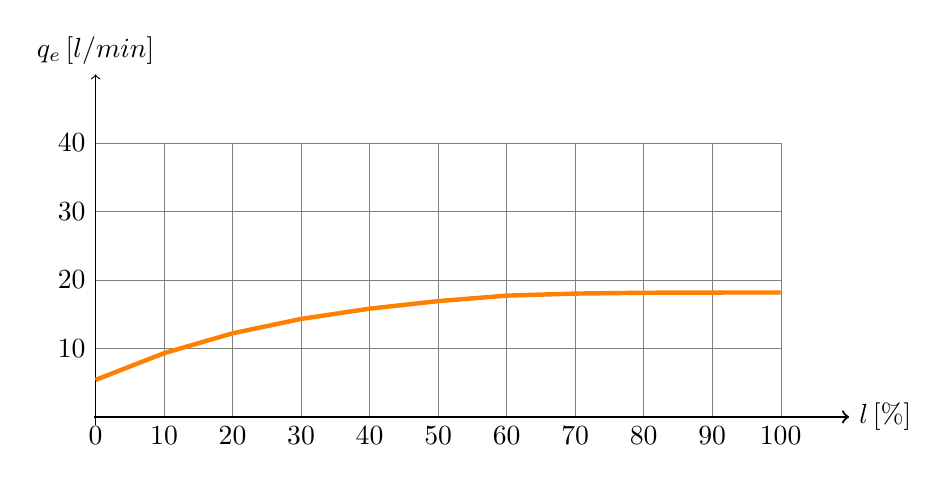
\begin{tikzpicture}[scale= 0.087, domain=0:110]
    
    \draw[ultra thin,color=gray,step=10cm] (100,40) grid (0.1,0.1);
    \draw[thick,->] (-0.2,0) -- (110,0) node[right,draw=none] {$l\,[\%]$};
    \draw[->] (0,-1.2) -- (0,50) node[above,draw=none] {$q_e\,[l/min]$};
    
    \foreach \x in {0,10,20,30,40,50,60,70,80,90,100}
    \draw (\x cm,1pt) -- (\x cm,-1pt) node[anchor=north,draw=none] {$\x$};
    \foreach \y in {10,20,30,40}
    \draw (1pt,\y cm) -- (-1pt,\y cm) node[anchor=east,draw=none] {$\y$};
    
    \draw[color = orange,ultra thick] (0,5.4) -- (10,9.3) -- (20,12.2)
    -- (30,14.3) -- (40,15.8) -- (50,16.9) -- (60, 17.7) -- (70, 18.0) 
    -- (80,18.12) -- (90,18.15) -- (100,18.16);
   
\end{tikzpicture}
\caption{Característica efectiva de la válvula con tiempo muerto}
\label{fig:valvulaCtiempoMuerto}
\end{figure}

\subsection{Efecto de flujo estrangulado}
\label{subsec:chokedflow}

Luego de analizar los resultados obtenidos en las pruebas de la planta, se pudo
constatar la presencia del efecto de flujo estrangulado o \emph{Choked
Flow}: se observa que la velocidad del fluido permanece constante a partir de
un valor determinado.
Posteriores incrementos de la carrera (y por ende, de la presión diferencial) no
aumentan la velocidad del fluido en la válvula.

Es una condición dinámica del fluido asociada con el efecto Venturi.
Cuando un flujo de fluido a una presión y temperatura dada pasa a través de una
restricción (por ejemplo: garganta, zona convergente/divergente o válvula),
la presión disminuye y la velocidad del fluido aumenta.
Si la presión desciende por debajo de la presión de vapor a la
temperatura del fluido, se da un fenómeno de evaporación violenta denominado
\emph{flashing}.
Las burbujas entorpecen el paso del líquido, limitando el caudal máximo
\cite{bib:controlValveHandbook,bib:ApuntesPuglesiValvulas}.

Además, si el fluido regresa a una presión superior a la presión de vapor luego
de pasar por la válvula, se obtiene el fenómeno de cavitación descripto en la
Sec. \ref{subsec:cavitacion}.
La cavitación, además de generar el efecto de flujo estrangulado, produce daños
en el conjunto asiento-obturador.

\subsection{Montaje}
Dada la importancia y tamaño de la válvula, se colocó en el centro de
la planta, sobre la base de madera. Se trató que se pudieran apreciar
con claridad las diferentes partes que la componen.
Se prestó especial atención al nivelado de la válvula.
Finalmente, se fijó mediante ménsulas a la base de madera y a la estructura
de caño.

\section{Instrumentación}
\label{sec:InstrumentosMedicion}
Para conocer el estado de la planta, es necesario tener conocimiento de varias
variables de la planta, a saber:
\begin{itemize}
 \item \textbf{Nivel de los tanques}
 \item \textbf{Caudal en las tuberías}
 \item \textbf{Presión en las tuberías}
\end{itemize}
Se deben instalar elementos de instrumentación, para poder
medir y controlar estas variables de interés.

\subsection{Manómetros}
\label{subsec:Manometros}

\begin{figure}[t]
        \centering
        \begin{subfigure}[b]{0.48\textwidth}
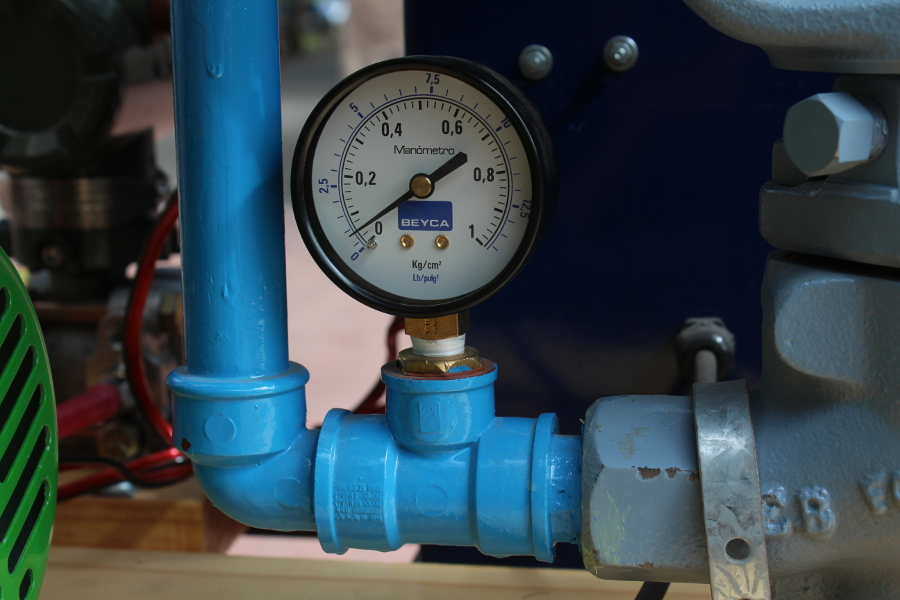
\includegraphics[width=\textwidth]
	{Cap2-DisenoEnsamblado/images/manometro1.JPG}
	%  TODO, cambiar foto por el nuevo
	\caption{Tubería de llenado, \texttt{PI 1}}
        \end{subfigure}%
        \hfill
        \begin{subfigure}[b]{0.48\textwidth}
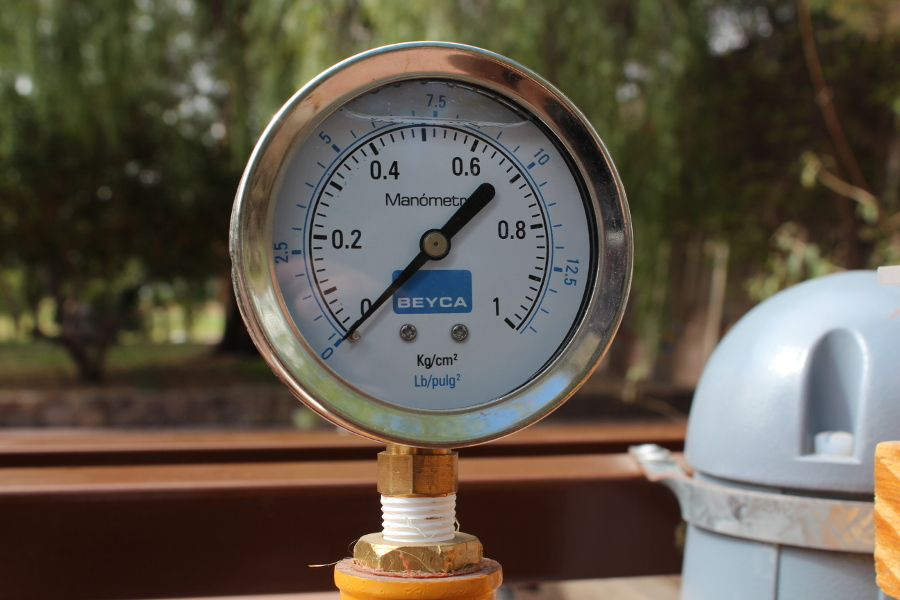
\includegraphics[width=\textwidth]
	{Cap2-DisenoEnsamblado/images/manometro2.JPG}
	\caption{Tubería de vaciado, \texttt{PI 2}}
        \end{subfigure}
        \caption{Manómetros en la planta}
        \label{fig:manometro}
\end{figure}

\begin{figure}[t]
 \centering
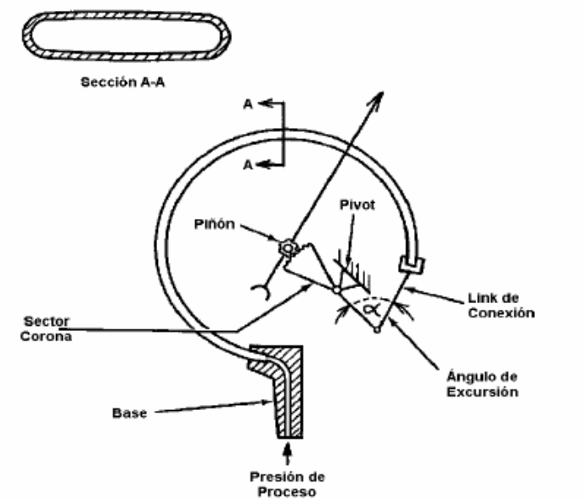
\includegraphics[width=.59\textwidth]
{Cap2-DisenoEnsamblado/images/manomBourdon.png}
 \caption{Manómetro de Bourdon, extraído de \cite{bib:ApuntesPuglesiPlacaOrif}}
 \label{fig:manometroBourdon}
\end{figure}

Para conocer los valores de presión en ambas tuberías
(referirse al \gls{pyid}, Sec. \ref{sec:p&id}),
se instalaron manómetros comunes, de tipo Bourdon.
Un ejemplo de estos manómetros se muestra en la Fig. \ref{fig:manometroBourdon}.
Se observa que un incremento de la presión produce una deformación
del \emph{tubo de Bourdon}, reflejado en la aguja indicadora.
El manómetro de Bourdon permite obtener una medición visual de la
presión relativa, del punto donde se encuentra instalado.



Durante el montaje, se observó que el manómetro de la tubería de vaciado
no entregaba una medición definida, sino que oscilaba alrededor de un
valor medio (imposibilitando la lectura directa).
Este problema fue solucionado instalando un \textbf{manómetro con glicerina},
donde el mecanismo del manómetro se encuentra sumergido en un baño de glicerina.
Debido a la viscosidad del fluido, las vibraciones quedan amortiguadas
y el manómetro refleja el valor medio de la presión.

Las especificaciones de los manómetros se muestran en la Tab.
\ref{tab:EspManoms}.

\begin{table}[h]
\renewcommand{\arraystretch}{1.3}
\centering
\begin{tabular}{|l|l|l|}
\hline
Manómetro & \texttt{PI 1}& \texttt{PI 2}\\
\hline
Marca & Cane & Beyca \\
Rango & $0$ - $7\,bar$ ($0$ - $100\,psi$) & $0$ - $1\,kgf/cm^2$ ($0$
- $14\,psi$) \\
Escala & $0.5\,bar/div$ ($2\,psi/div$) & $0.02\,kgf/cm^2/div$
($0.5\,psi/div$)\\
\hline
\end{tabular}
\caption{Especificaciones de los manómetros}
\label{tab:EspManoms}
\end{table}

En la Fig. \ref{fig:manometro} se observan los dos manómetros
presentes en el proyecto.

\subsection{DP Cell}
\label{subsec:DPCell}

Se denomina \textit{DP Cell}, o celda de presión diferencial, a un transductor
asociado a un transmisor de señal
que mide la diferencia de presión entre dos puntos.
En este caso, la celda entrega una corriente proporcional a la diferencia de
presión medida, en el rango de $4-20\,mA$.
Este valor de corriente es leído por el controlador de la planta.

Las DP cell utilizadas tienen las especificaciones que se muestran en la Tab.
\ref{tab:caractDPcell}.

\begin{table}[ht]
\renewcommand{\arraystretch}{1.3}
\centering
\begin{tabular}{|l|l|}
\hline
Marca & Yokogawa\\
Modelo & EJA 110 A\\
Sufijo & EMSOA - 22EN / FU1 / D4\\
Tensión & $10.5\,-\,30 \, DC$\\
Output & $4-20\,mA$\\
Presión máxima & $160\,bar$\\
Rango de calibración & $0$ a $10000\,mmCa$\\
\hline
\end{tabular}
\caption{Especificaciones de las celdas de presión diferencial}
\label{tab:caractDPcell}
\end{table}

Dos celdas son utilizadas:
\begin{itemize}
 \item \textbf{Medición del nivel del tanque:} la entrada de alta presión de la
celda
se conecta  al nivel más bajo del tanque y la de baja se deja desconectada
(presión atmosférica).
La celda mide la presión debida al peso de la columna de agua en el tanque.
Fue calibrada de manera que entregara un valor de corriente mínimo
cuando el tanque está vacío, y un valor máximo en el caso de que esté
lleno.
Así, el valor entregado por la celda es proporcional al nivel de
agua en el tanque.

\item \textbf{Medición del caudal en la tubería de llenado del tanque
controlado:}
Se utilizó una placa orificio para generar una caída de presión debida al
caudal.
Las entradas de la celda se conectan aguas arriba y aguas abajo
de la placa orificio.
Se mide de esta manera la diferencia de presión entre ambos puntos, que será
traducido en un valor de caudal en el
controlador (ver Sec. \ref{subsec:PlacaOrificio}).
\end{itemize}

Ambas celdas fueron fijadas a la base de madera mediante tornillos.
Las conexiones de las entradas se realizaron con tuberías flexibles de alta
presión malladas, de $6\,mm$. Se muestran en la Fig. \ref{fig:dpcelfig}.

\begin{figure}[t]
        \centering
        \begin{subfigure}[b]{0.31\textwidth}
        \centering
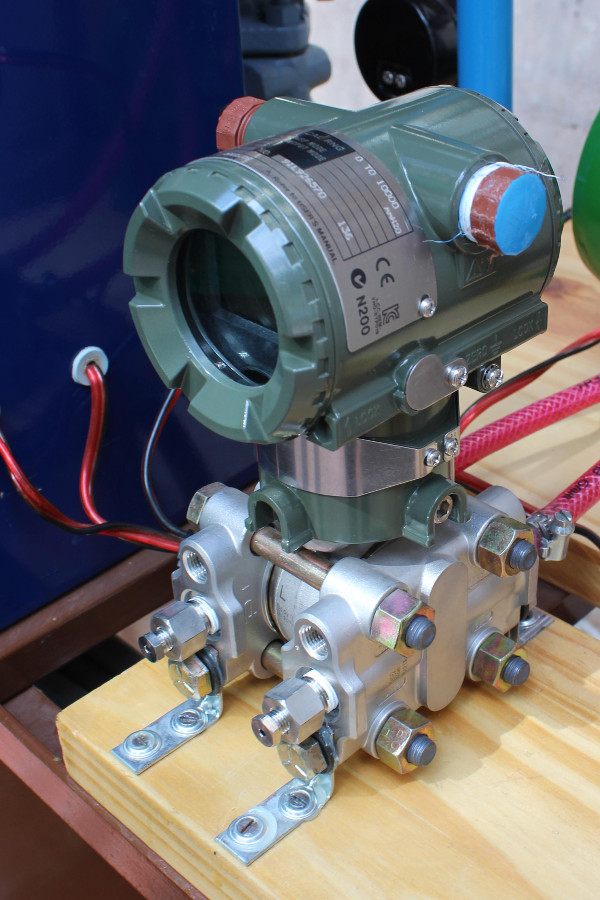
\includegraphics[height=6.3cm]
	{Cap2-DisenoEnsamblado/images/dpcell1.JPG}
	\caption{Vista general}
        \end{subfigure}%
        \hfil
        \begin{subfigure}[b]{0.69\textwidth}
        \centering
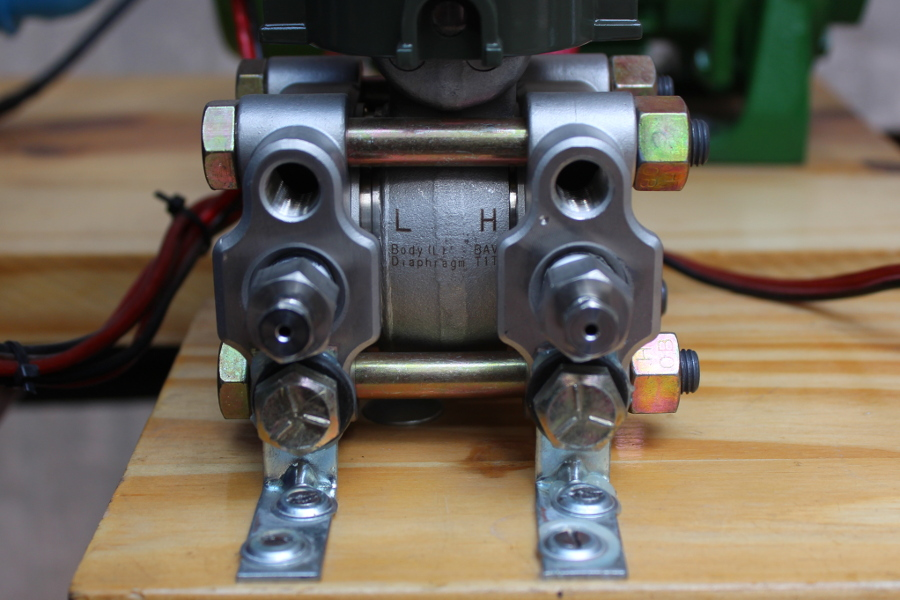
\includegraphics[height=6.3cm]
	{Cap2-DisenoEnsamblado/images/dpcell2.JPG}
	\caption{Detalle tomas de baja y alta presión}
        \end{subfigure}
        \caption{DP cells en la planta}
        \label{fig:dpcelfig}
\end{figure}

Se debe destacar que, para el caso de la celda de caudal, ambas
entradas se conectaron entre si mediante una válvula manual.
Esta válvula se utiliza solamente durante el primer arranque de la planta:
cuando la tubería está vacía y la electrobomba \verb|B1| se activa, se tiene por
una pequeña
fracción de tiempo una presión diferencial de $12\,mCa$ que puede dañar la
celda.
Para evitar este fenómeno, la válvula manual que conecta ambas entradas
permanece abierta durante el primer arranque.
Luego, debe cerrarse para poder realizar la lectura diferencial de presión.

\subsection{Placa orificio}
\label{subsec:PlacaOrificio}


\begin{figure}[t]
 \centering
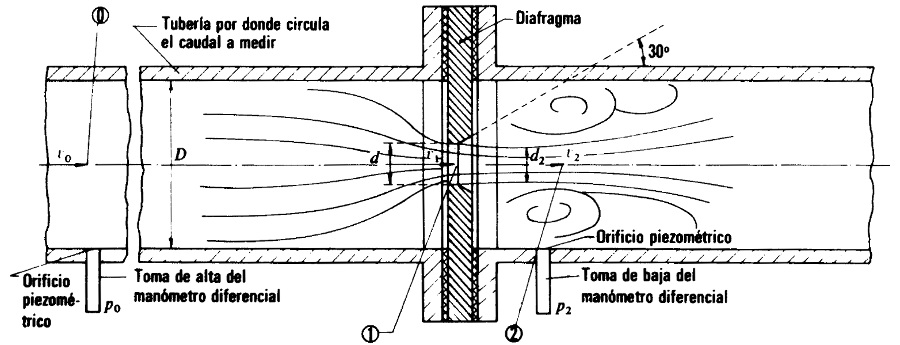
\includegraphics[width=\textwidth]{Cap2-DisenoEnsamblado/images/placaOrif.png}
\caption{Corte longitudinal de una placa orificio montada en una tubería
\cite{bib:Mataix}}
 \label{fig:placaOrificio}
\end{figure}

Para medir el caudal en la tubería de llenado, se decide
utilizar una placa orificio.
En la Fig. \ref{fig:placaOrificio} se muestra un
corte longitudinal de la misma.
Se observa que la placa orificio provoca una disminución del diámetro
de la tubería, con la consiguiente aceleración del fluido y disminución de la
presión.
Puede medirse una diferencia de presión entre un punto aguas arriba y un punto
próximo a la placa orificio, aguas abajo.
Se describe a continuación la expresión para obtener el caudal que circula en
la tubería, a partir de la medición de la presión diferencial.

Escribiendo la ecuación de Bernoulli en 0 y 2, considerando que la velocidad en
2 es aproximadamente igual a la velocidad en 1,
\begin{align}
 z_0 \, \gamma + \dfrac{\rho \,v_0^2}{2} + P_0 &= z_2 \, \gamma + \dfrac{\rho
\,v_2^2}{2} + P_2
\label{eq:Bernoulli}
\end{align}
donde $z_i$ y $P_i$ es la altura y presión en el punto $i$ y $\rho$ es 
la densidad del fluido.
Considerando que la altura en ambos puntos es la misma, la ecuación
\eqref{eq:Bernoulli} puede reescribirse como
\begin{align}
 v_2^2 - v_0^2 &= 2\,g\,h_p
 \label{eq:Bernoulli2}
\end{align}
donde $h_p$ es la diferencia de presión entre 0 y 2, expresada como
altura de la columna fluida
\begin{align}
 h_p &= \dfrac{P_0}{\gamma}-\dfrac{P_2}{\gamma}
\end{align}

La ecuación de continuidad, para fluidos incompresibles se escribe
\begin{align}
 A_2\,v_2 &= A_0\,v_0 \\
% D_2^2\,v_2 &= D_0^2\,v_0\\
 v_2 &= \dfrac{D_0^2}{D_2^2} v_0
 \label{eq:velRef}
\end{align}
y reemplazando \eqref{eq:velRef} en \eqref{eq:Bernoulli2} se obtiene
\begin{align}
 2 \, g \, h_p &= v_2^2 \left( 1 - \dfrac{D_0^4}{D_2^4} \right)\\
 \beta &= \dfrac{D_0}{D_2}\\
 v_2 &= \sqrt{\dfrac{2 \, g \, h_p}{1-\beta^4}}
\end{align}
finalmente, el caudal se obtiene multiplicando la velocidad $v_2$ por el
área $A_2$.
Además, se agrega un coeficiente $C_v$ debido al fenómeno de vena contracta:
\begin{align}
 Q &= \dfrac{C_v \, A_2}{\sqrt{1-\beta^4}}\, \sqrt{2 \, g \, h_p}
 \label{eq:placaOrif1}
\end{align}

El coeficiente $C_v$ depende del número de Reynolds $Re$
\cite{bib:Mataix, bib:ApuntesPuglesiPlacaOrif}
\begin{align}
Re &= \dfrac{D\,v}{\nu}
\end{align}
donde $v$ es la velocidad en la placa orificio, $D$ es el diámetro y ${\nu}$
es la viscosidad cinemática del fluido\footnote{Para el agua, el fluido de
trabajo utilizado $\nu = 1,003\,10^{-6} \frac{m^2}{s}$.}.

La ecuación \eqref{eq:placaOrif1} puede ser reescrita de una forma más sencilla
mediante una nueva variable adimensional $C_q$
\begin{align}
 C_q &= \dfrac{C_v}{\sqrt{1-\beta^4}}
\end{align}
$C_q$, por consiguiente depende tanto del número de Reynolds como de la razón
de los diámetros $\beta$. $C_q$ puede ser encontrado en tablas y ábacos en la
literatura \cite{bib:Mataix}.

No obstante, se observa que el valor de $C_q$ varia poco para valores de
$Re > 20000$, y depende fundamentalmente de $\beta$.
Por ende, puede ser considerado constante para una instalación dada.
Finalmente, la ecuación \eqref{eq:placaOrif1} puede ser expresada como
\begin{align}
 Q &= C_q\,A_2\, \sqrt{2\,g\,h_p}
\end{align}
que puede ser reescrita, teniendo a $C_q$ constante
\begin{align}
 Q &= K\,\sqrt{h_p}
 \label{eq:placaOrifPLC}
\end{align}
donde se observa que el caudal $Q$ es proporcional a la raíz cuadrada de
la diferencia de alturas $\sqrt{h_p}$, que puede
ser encontrada utilizando un DP cell (ver Sec. \ref{subsec:DPCell}).

\subsubsection{Montaje}
La placa orificio se colocó en serie con la tubería de llenado del
tanque controlado.
Debieron instalarse además, las tuberías flexibles correspondientes de conexión
con la celda de presión diferencial.

\subsubsection{Metodología experimental}
Considerando $C_q$ constante,
\begin{align}
 K = C_q\, A_2\, \sqrt{2\,g}
\end{align}
es constante también, y puede ser determinado experimentalmente.
Para ello, se midió sobre el tanque controlado una distancia $l$.
Luego, se encendió la electrobomba \verb|B1| con la válvula de control en
posición
abierta (caudal máximo), y se midió el tiempo $t$ necesario para que el nivel
alcanzara la altura $l$.
Ya que el tanque tiene un diámetro $D$, el caudal máximo puede ser
calculado como
\begin{align}
 Q_{max} &= \dfrac{\pi\,D^2\,l}{4\,t}
\end{align}

El módulo analógico del \gls{plc} tiene una resolución de $12\,bits$
(ver Sec. \ref{subsec:plc}), un valor de caudal máximo corresponde a $h_f =
4095$.
$K$ se calcula como
\begin{align}
 K &= \dfrac{Q_{max}}{\sqrt{4095}}
\end{align}
Luego, el caudal puede calcularse fácilmente aplicando la ecuación
\eqref{eq:placaOrifPLC}.

Para la determinación del valor de $K$ se trabajó sin tiempo muerto.
Se marcó en el tanque controlado una altura $l=0.5\,m$, teniendo $D=0.2\,m$.
Luego, se procedió a medir el tiempo de llenado, consignando los resultados en
la Tab. \ref{tab:tiempoK}.

\begin{table}[ht]
\renewcommand{\arraystretch}{1.3}
  \centering
  \bgroup
%   \scriptsize
%   \def\tabcolsep{6.50pt}
%   \def\arraystretch{1.22}%
  \begin{tabular}{|c|c|}
  \hline
  Medición & Valor\\
  \hline
  1 & $27.27\,s$ \\
  2 & $28.53\,s$ \\
  3 & $27.98\,s$ \\
  4 & $28.10\,s$ \\
  5 & $27.68\,s$ \\
  6 & $27.66\,s$ \\
  \hline
  \hline
  \textbf{Media} & $27,87\,s$\\
  \textbf{SD} & $0.43\,s$\\
  \hline
  \end{tabular}
  \egroup
  \caption{Medición del tiempo de llenado, cálculo de $K$}
  \label{tab:tiempoK}
\end{table}

Finalmente, se obtiene
\begin{align}
 Q_{max} &= 33.81\,\dfrac{lts}{min}
 \\
 K  &= 0.5285\,\dfrac{lts}{min}
\end{align}

\section{Planta ensamblada}
Se presenta la planta ensamblada en la Fig. \ref{fig:PlantaEnsamblada}, vista
desde el lado de la válvula.
Pueden observarse claramente la estructura, la distribución de los elementos,
las tuberías de llenado y vaciado, las tuberías flexibles de conexión a las DP
Cell, el tiempo muerto y los tanques.

\begin{figure}[ht]
	\centering
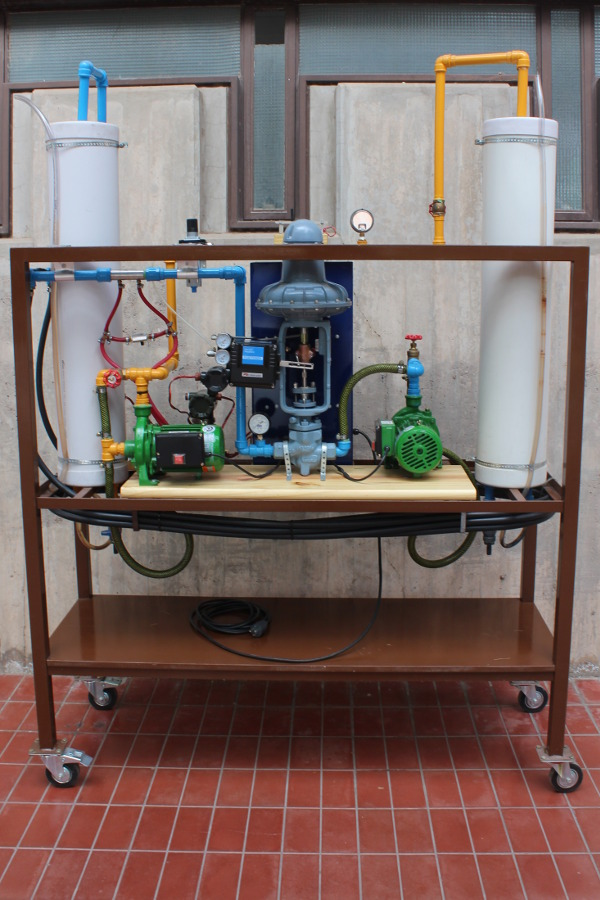
\includegraphics[width=.94\textwidth]{Cap2-DisenoEnsamblado/images/IMG_5123.JPG}
	\caption{Planta ensamblada}
	\label{fig:PlantaEnsamblada}
\end{figure}

% REVISIÓN 1 - fclad
